\chapter{Experiments and results}

This chapter describes the experiments we performed to show the effectiveness of the proposed method. 

\section{Evaluation datasets}
To quantitatively evaluate the proposed methods, and to compare it to related work,
we considered two datasets: the DSO-1 and DSI-1 datasets\footnote{Public available for download at https://recodbr.wordpress.com/code-n-data}. Each dataset comes with a face position groundtruth and a splicing mask. Additionally, the ColorChecker dataset \cite{gehler2008bayesian} is used as a source of pristine images.


This dataset has been mainly used for experimenting on pristine data: due its characteristics is very varied and lends itself well to image analysis based on color.

\subsection{DSO-1}

The DSO-1 dataset is composed of 200 indoor and outdoor images with image resolution of 2048 × 1536 pixels. Out of this set of images, 100 are original, i. e., have no adjustments whatsoever, and 100 are forged. 

\begin{figure}[!htb]
\minipage{0.48\textwidth}
  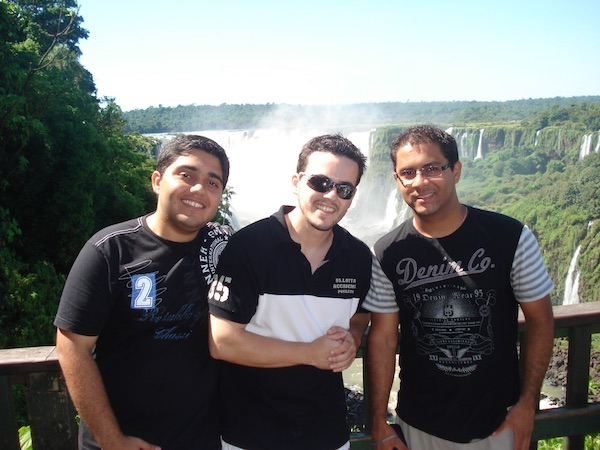
\includegraphics[width=\linewidth]{dso_sample}
  \caption{DSO-1 sample original image}\label{fig:dsooriginalimage}
\endminipage\hfill
\minipage{0.48\textwidth}
  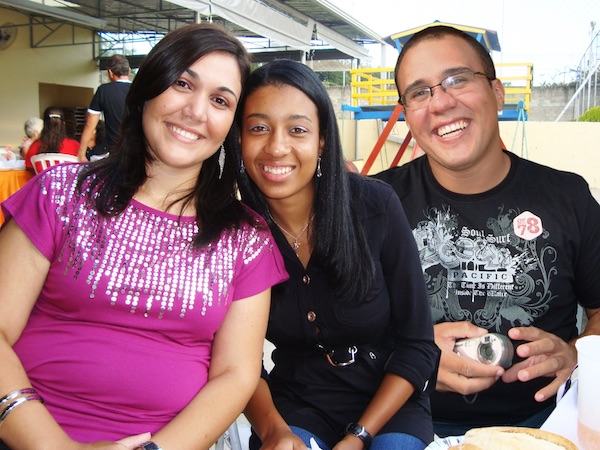
\includegraphics[width=\linewidth]{dso_sample_spliced}
  \caption{DSO-1 sample spliced image}\label{fig:dsosplicedimage}
\endminipage
\end{figure}

The forgeries were created by adding one or more individuals in a source image that already contained one or more people. When necessary, we complemented an image splicing operation with post-processing operations (such as color and brightness adjustments) in order to increase photorealism.

\subsection{DSI-1}

The DSI-1 dataset is composed of 50 images (25 original and 25 doctored) downloaded from different websites in the Internet with different resolutions. Original images were downloaded from Flickr and doctored images were collected from different websites such as Worth 1000, Benetton Group 2011, Planet Hiltron, etc.

\begin{figure}[!htb]
\minipage{0.46\textwidth}
  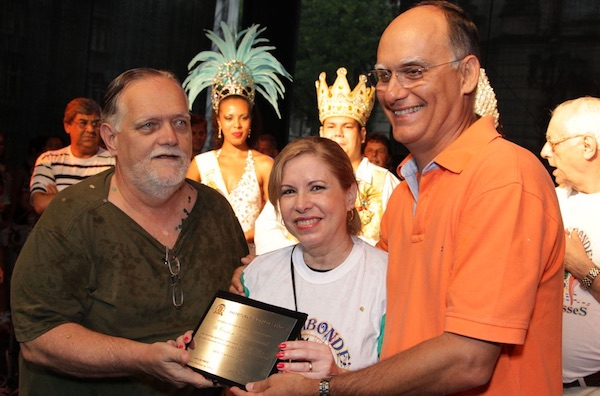
\includegraphics[width=\linewidth]{dsi_sample_normal}
  \caption{DSI-1 sample original image}\label{fig:dsioriginalimage}
\endminipage\hfill
\minipage{0.50\textwidth}
  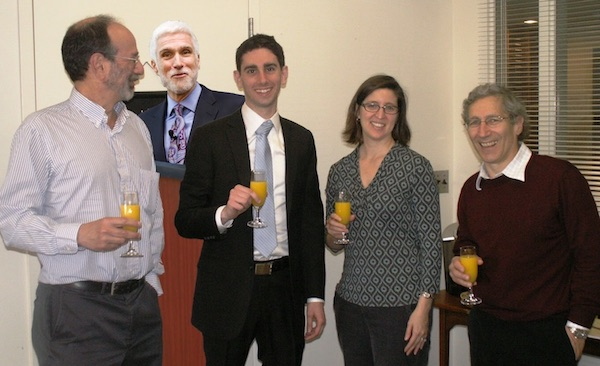
\includegraphics[width=\linewidth]{dsi_sample_spliced}
  \caption{DSI-1 sample spliced image}\label{fig:dsisplicedimage}
\endminipage
\end{figure}

\subsection{ColorChecker}

The ColorChecker dataset is a collection of images for evaluating Color Constancy algorithms built as additional material to \cite{gehler2008bayesian}. It consists in 568 RGB colored images of different scenes, both indoor and outdoor taken under different illuminations. In each scene a Gretag MacBeth Color Checker Chart was placed such that it was illuminated by the main scene illuminant and thus its color could be retrieved. The data is available in Canon RAW format free of any correction.

\begin{figure}[h!]
  \centering
    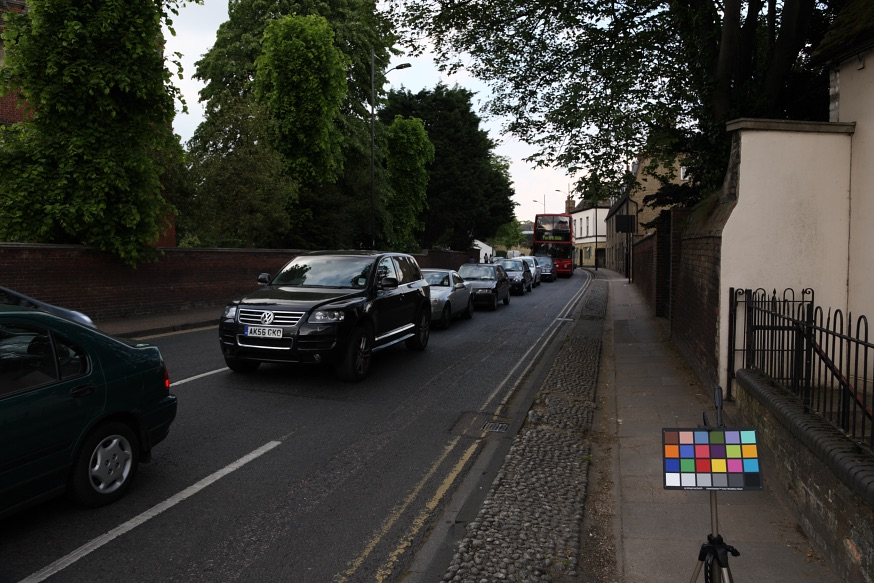
\includegraphics[width=0.65\textwidth]{colorchecker_sample}
    \caption{Example of an image of the ColorChecker dataset}
    \label{fig:colorcheckersample}
\end{figure}

\section{Face forgery detection module performance}

This section describes the experiments performed to evaluate the face forgery detection module. In these experiments, the DSO-1 and the DSI-1 datasets are used for evaluation.

After characterizing an image with a specific image descriptor, the next step consists of using an appropriate learning method.

the proposed method method focuses on using complementary information, the color descriptors, to describe the Illuminant Maps. Accordingly to Carvalho \emph{et al. }\cite{carvalho2016illuminant}, we selected the k-Nearest Neighbor (kNN) classifier instead of more powerful and computational intensive ones such as Support Vector Machines (SVM) due fact that, SVM and kNN, or even fusion of both learning methods, present very similar results, enforcing the choice for a simpler learning technique (kNN)\cite{carvalho2016illuminant}. The value of \emph{k} is set to 5. 

For all image descriptors, we have used the standard con- figuration proposed by \emph{Penatti et al.} \cite{penatti2012comparative}.

As described in Chapter 2, eight different kNN models are trained and used for the classification, considering all the possible combinations of the couples composed by a IMs transformed space (GGE e IIC)and a color descriptor (chosen from ACC, BIC, CCV and LCH).

\subsection{Color descriptors accuray}

Since the final classification output is given by majority voting of all the selected classifiers, the first round of experiments aimed at evaluating the accuracy of each image descriptors.

\begin{table}[h!]
\centering
\begin{tabular}{l c c c c c c} 
\hline \hline 
\textbf{Test case} & \textbf{Train} & \textbf{Test} & \textbf{ACC} & \textbf{BIC} & \textbf{CCV} & \textbf{LCH} \\ [0.5ex]
\hline
Test 1 & DSO-1 & DSO-1 &	0.75 & 0.75	& 0.72 & \textbf{0.78}\\
Test 2 & DSI-1 & DSI-1 &	0.78 & 0.79 & 0.77 & \textbf{0.82}\\
Test 3 &	DSO-1 &	DSI-1 &	0.56 & \textbf{0.57} & 0.53 & 0.53\\
Test 4 &	DSI-1 & DSO-1 & 0.58 & 0.55 & 0.51 & \textbf{0.59}\\ [1ex]
\hline
\end{tabular}
\caption{Accuracy for kNN technique using a single color descriptor. Experiments are performed using 10-fold cross-validation in test case number 1 and 2.}
\label{table:colordescriptorperformance}
\end{table}

Table \ref{table:colordescriptorperformance} shows the results of all tested combinations of train and test set. The classification results show that, generally, LCH color descriptor yielded the higher accurary, but there is not a descriptor that outperforms the others.

\subsection{Test cases}

After analyzing each single descriptor accuracy, we proceeded to evaluate the overall module using a combination of all of them, as described in Chapter 2. Since not all the color descriptors perform equally, a different weight is given at each classifier.


In the following experiments, the  method has been applied for classifying a face pair as fake or real using uniform (Table \ref{table:performancefacedet}) and non-uniform (Table \ref{table:performancefacedetnonun}) weights. Essentially, these experiments evaluate the forgery detection performances.

For each test case in the suite it is reported:
\begin{enumerate}
\item The training dataset (\textbf{\emph{Train}});
\item The evaluation dataset (\textbf{\emph{Test}});
\item The classification accuracy score (\textbf{\emph{Accuracy}});
\item The area under the R\emph{eceiver Operator Characteristic (ROC)} curve (\textbf{\emph{AUC}})
\item The accuracy score expressed through the $F_1$ score (also known as \textbf{\emph{F-Score}})
\end{enumerate}

Accordingly with \emph{Jeni et al.} \cite{jeni2013facing}, when dealing with AUC score to measure the performance of classifier, one of the major drawbacks relies on the fact that an increasing of AUC doesn't really mean a better classifier, but it could be just the side-effect of too many negative examples used in training.

Therefore, also another classification accuracy score is provided, the \emph{F-Score}. Given $TP$, $FP$ and $FN$ the true positives, false positives and false negatives values. 

Let the classification \emph{precision} score given by

$$
precision = \frac{TP}{TP + FP}
$$

where $TP$ and $FP$ are true positives and false positives respectively.

The \emph{recall} value is defined as
$$
recall = \frac{TP}{TP + FN}
$$
where $FN$ stands for false negatives. The $F_{\beta}$ score is defined as the harmonic mean of precision and recall values:

\begin{equation}
F_{\beta} = (1 + \beta^2) * \frac{precision * recall}{(\beta^2 * precision) + recall}
\end{equation}

where $\beta$ states for the relative importance given to precision comparing to recall. In our experiments, we considered $\beta = 1$ (i.e. the $F_1$ score), so:
\begin{equation}
F_{1} = 2 * \frac{precision * recall}{precision + recall}  = \cdots = \frac{2 * TP}{2 * TP + FP + FN}
\end{equation}

In order to proceed with the comparison between using uniform and non-uniform weights for classifiers, we have to determine the most appropriate weight values for each descriptor. The weights have been found with an exhaustive search by evaluating the performance of the currently analyzed weights combination over the DSO-1 dataset with a 10-fold cross-validation protocol. 

To reduce the computational cost, we limited the range of values to be explored for each classifier basing on the results reached for each single descriptor, presented in Table \ref{table:colordescriptorperformance}, giving more importance to LCH descriptor.

Experimental results are collected in Table \ref{table:performancefacedet}, for the uniform weights case, and in Table \ref{table:performancefacedetnonun}, for non-uniform case. 

\begin{table}[h!]
\centering
\begin{tabular}{l c c c c c} 
\hline \hline 
\textbf{Test case} & \textbf{Train} & \textbf{Test} & \textbf{ACC} & \textbf{AUC} &\textbf{ F-Score} \\ [0.5ex]
\hline
Test 1 & DSO-1 & DSO-1 &	0.82 & 0.88	& 0.77\\
Test 2 & DSI-1 & DSI-1 &	0.87 & 0.92 & 0.87\\
Test 3 &	DSO-1 &	DSI-1 &	0.58 & 0.58 & 0.62\\
Test 4 &	DSI-1 & DSO-1 & 0.62 & 0.59 & 0.53\\ [1ex]
\hline
\end{tabular}
\caption{Performance of face forgery detection module over paired faces using uniform weights.}
\label{table:performancefacedet}
\end{table}

\begin{table}[h!]
\centering
\begin{tabular}{l c c c c c} 
\hline \hline 
\textbf{Test case} & \textbf{Train} & \textbf{Test} & \textbf{ACC} & \textbf{AUC} &\textbf{ F-Score} \\ [0.5ex]
\hline
Test 1 & DSO-1 & DSO-1 &	0.84 & 0.90	& 0.78\\
Test 2 & DSI-1 & DSI-1 &	0.89 & 0.92 & 0.89\\
Test 3 &	DSO-1 &	DSI-1 &	0.59 & 0.58 & 0.64\\
Test 4 &	DSI-1 & DSO-1 & 0.63 & 0.60 & 0.54\\ [1ex]
\hline
\end{tabular}
\caption{Performance of face forgery detection module over paired faces using non-uniform weights.}
\label{table:performancefacedet}
\end{table}

Resulting accuracy scores are obtained as average over 5 consecutive runs of the algorithm. 

\begin{figure}[h!]
  \centering
    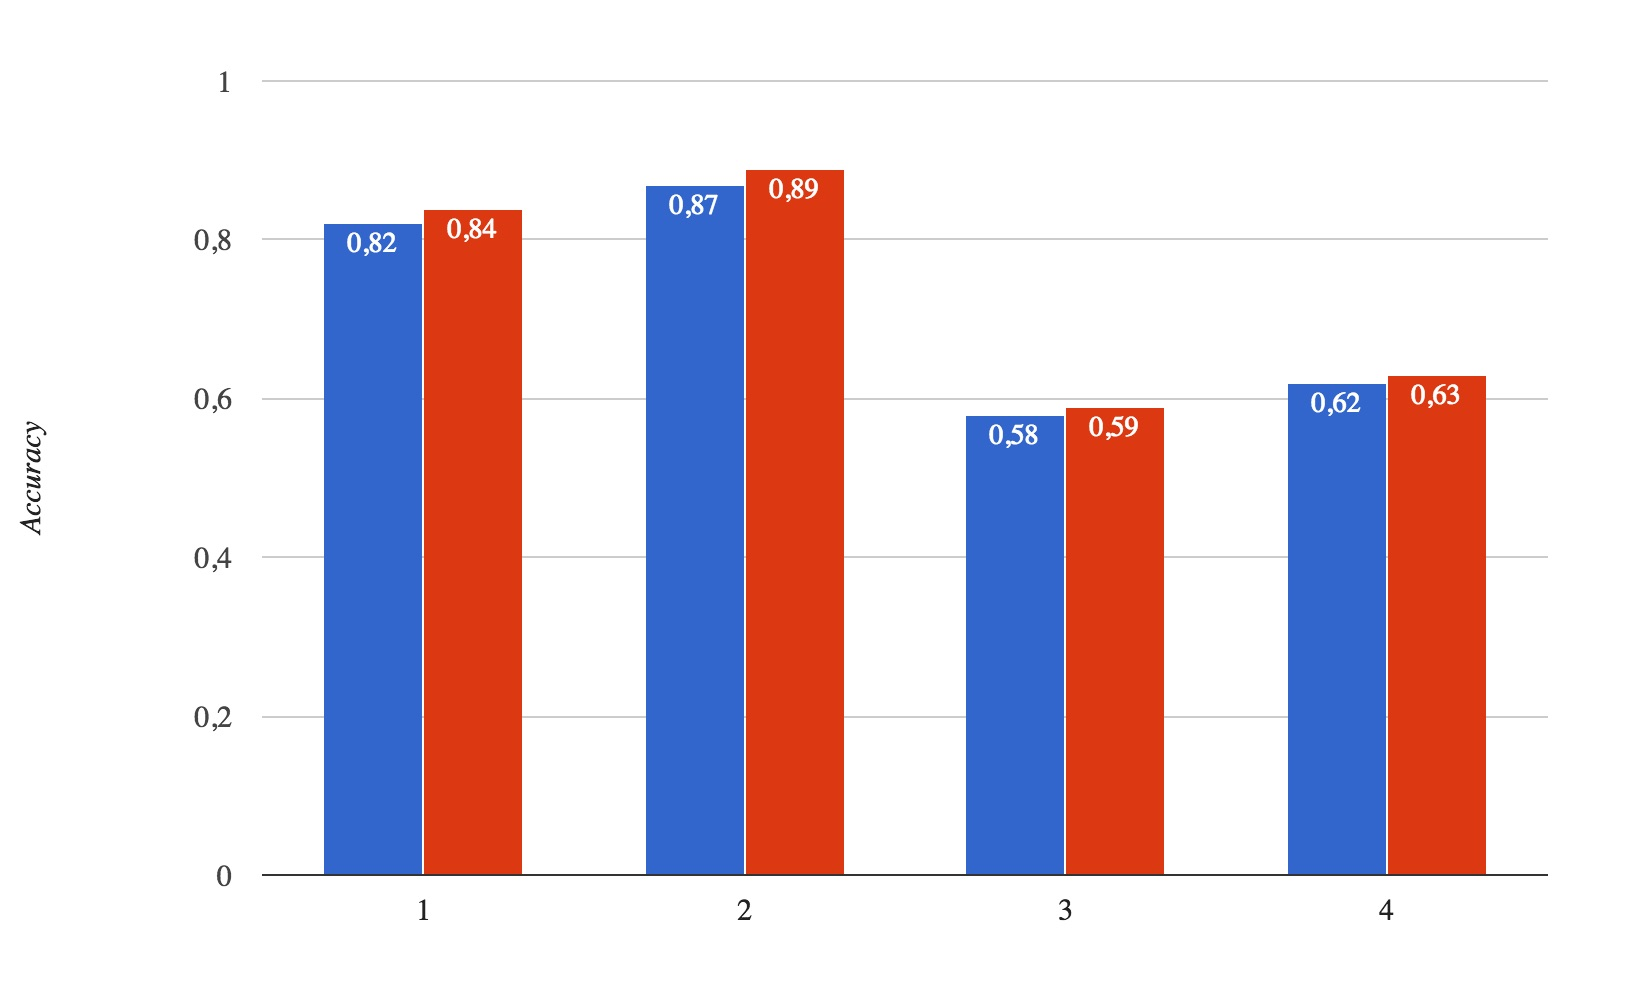
\includegraphics[width=0.9\textwidth]{compareknnweights}
    \caption{Classification accuracies comparison between using uniform and non uniform weights for kNN classifiers over the considered 4 test cases of Table \ref{table:performancefacedet}. The blue bins depict the reached accuracies using uniform weights, reds are for non-uniform case.}
    \label{fig:compareknnweights}
\end{figure}

These results show that, although we can notice a slight performance improvement in all test cases, the use of non-uniform weights do not affect much on the final classification results.

In the following subsections are described the experimental results for each analyzed test case. We show results using classical \emph{Receiver Operator Characteristic (ROC)} \cite{fawcett2006introduction} and Precision-Recall curves\cite{Davis:2006:RPR:1143844.1143874}. 

\subsubsection{Test case 1: performance on DSO-1 dataset}


\begin{figure}[h!]
  \centering
    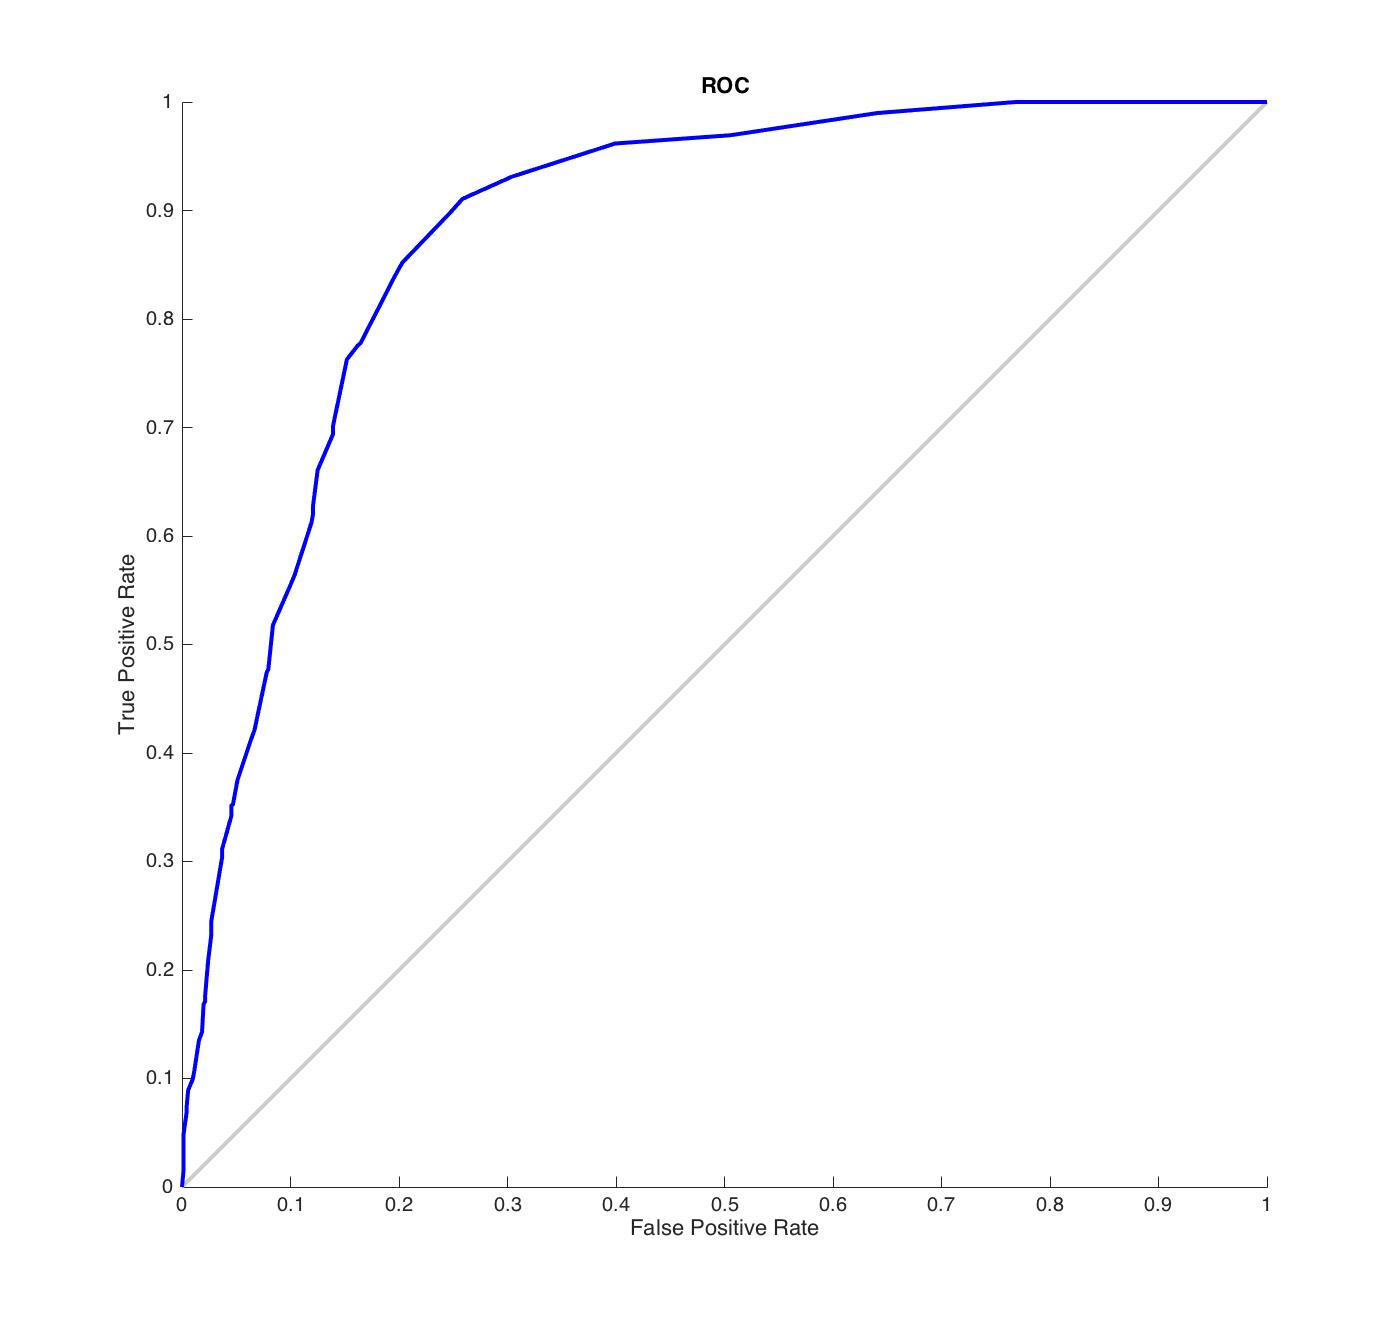
\includegraphics[width=0.85\textwidth]{train_dso_crossvalidation}
    \caption{The ROC curve  for DSO-1 cross-validation}
    \label{fig:train_dso_crossvalidation}
\end{figure}

\begin{figure}[h!]
  \centering
    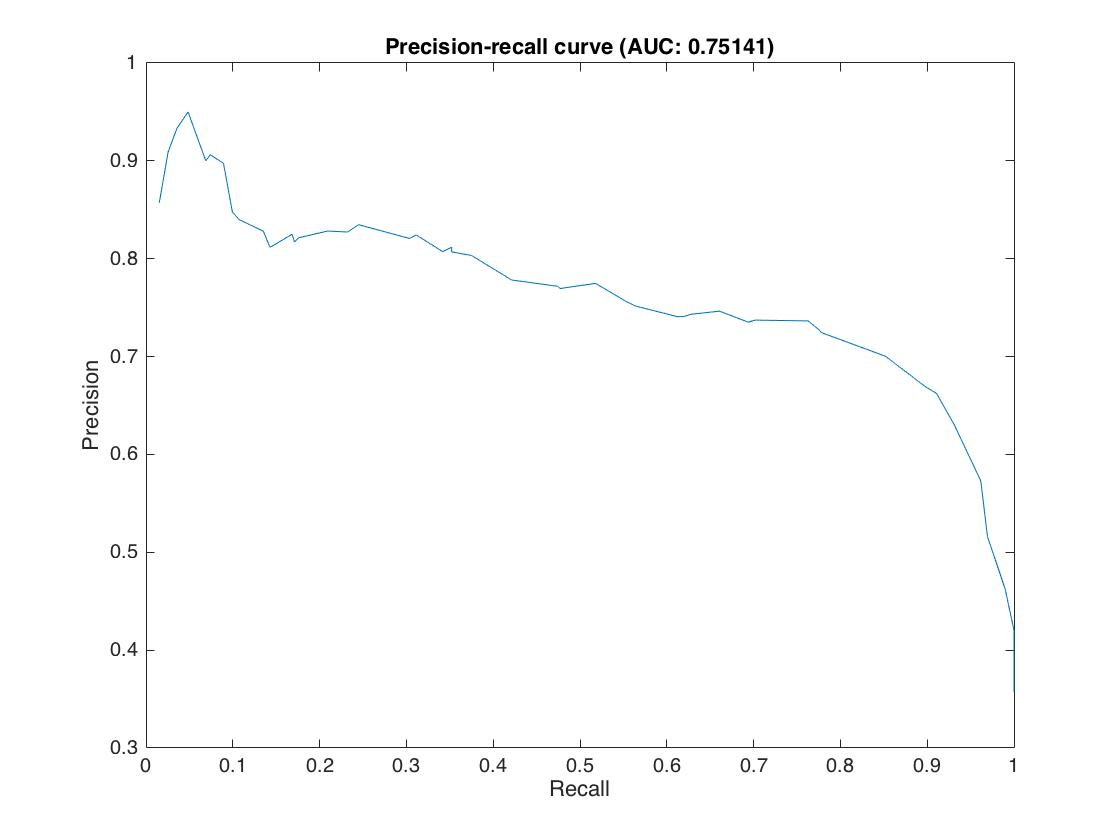
\includegraphics[width=0.85\textwidth]{train_dso_crossvalidation_prec_rec}
    \caption{The Precision-Recall curve for DSO-1 cross-validation}
    \label{fig:train_dso_crossvalidation_prec_rec}
\end{figure}

\subsubsection{Test case 2: performance on DSI-1 dataset}

\begin{figure}[h!]
  \centering
    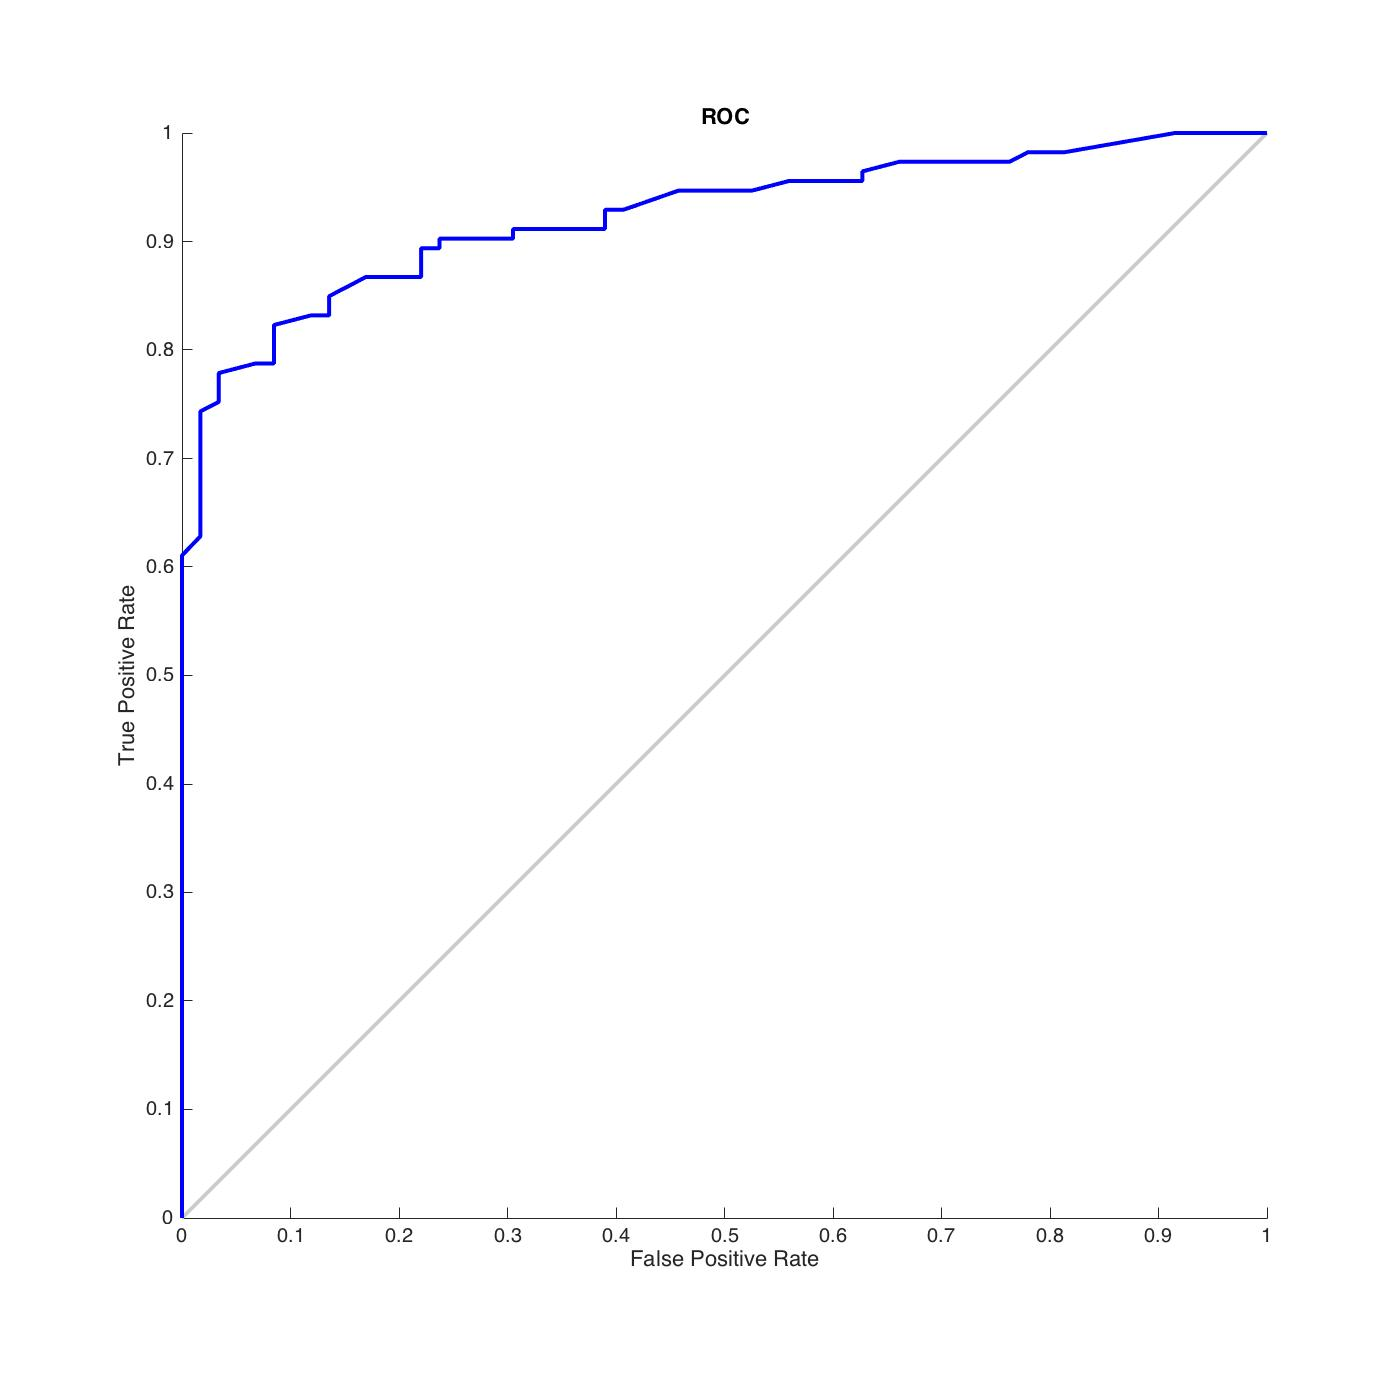
\includegraphics[width=0.85\textwidth]{train_dsi_crossvalidation}
    \caption{The ROC curve  for DSI-1 cross-validation}
    \label{fig:train_dsi_crossvalidation}
\end{figure}

\begin{figure}[h!]
  \centering
    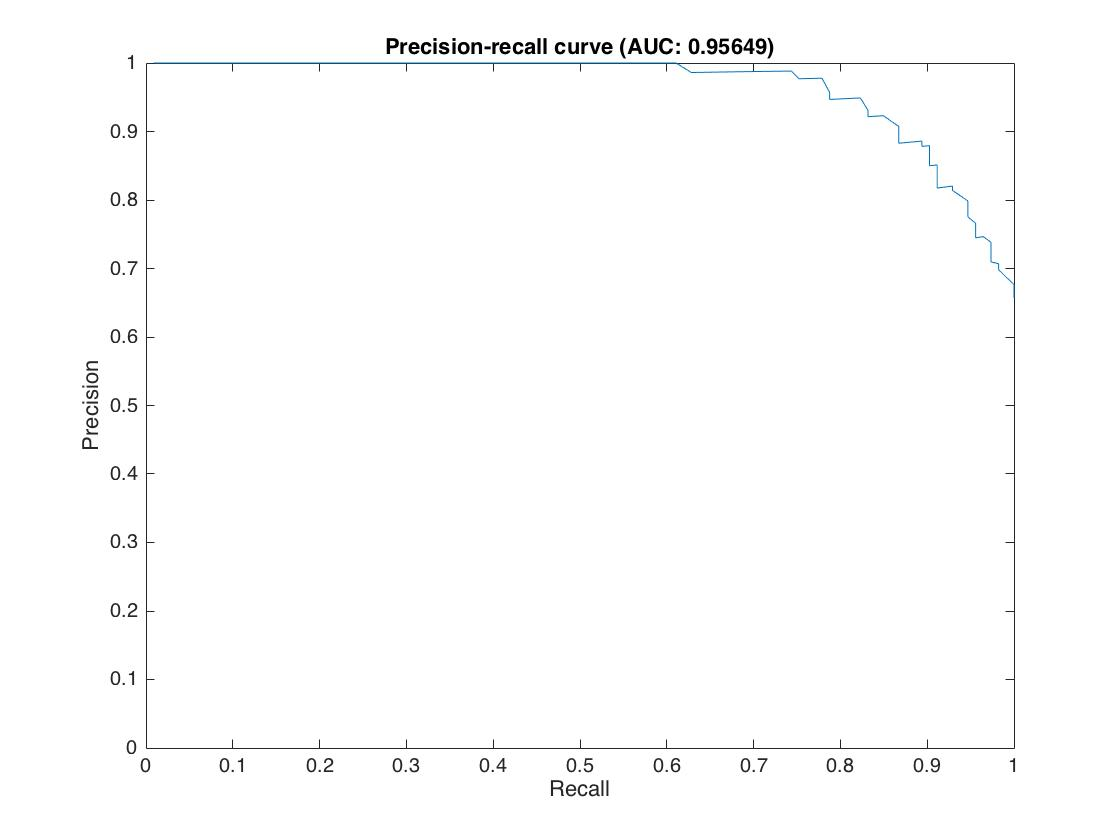
\includegraphics[width=0.85\textwidth]{train_dsi_crossvalidation_prec_rec}
    \caption{The Precision-Recall curve for DSI-1 cross-validation}
    \label{fig:train_dsi_crossvalidation_prec_rec}
\end{figure}

\subsubsection{Test case 3: cross dataset performance on DSO-1}

\begin{figure}[h!]
  \centering
    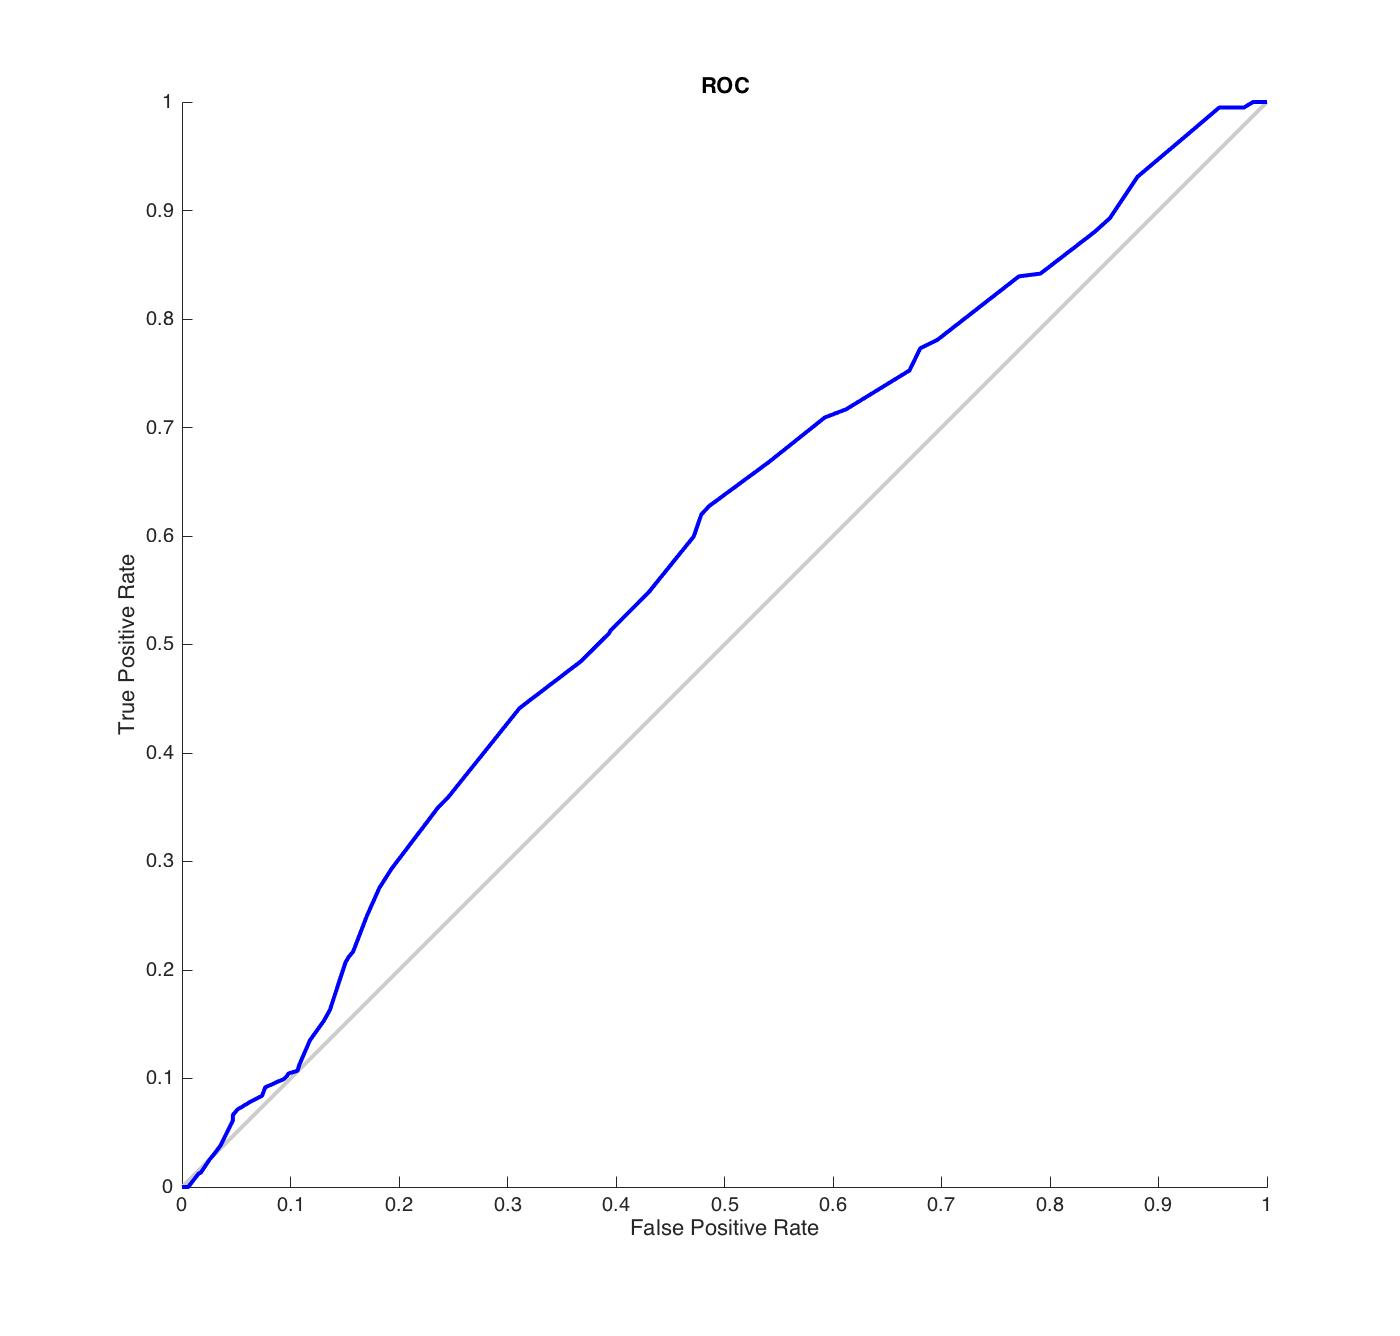
\includegraphics[width=0.85\textwidth]{train_dsi_test_dso}
    \caption{The ROC curve  for DSO-1 cross-validation}
    \label{fig:train_dsi_test_dso}
\end{figure}

\begin{figure}[h!]
  \centering
    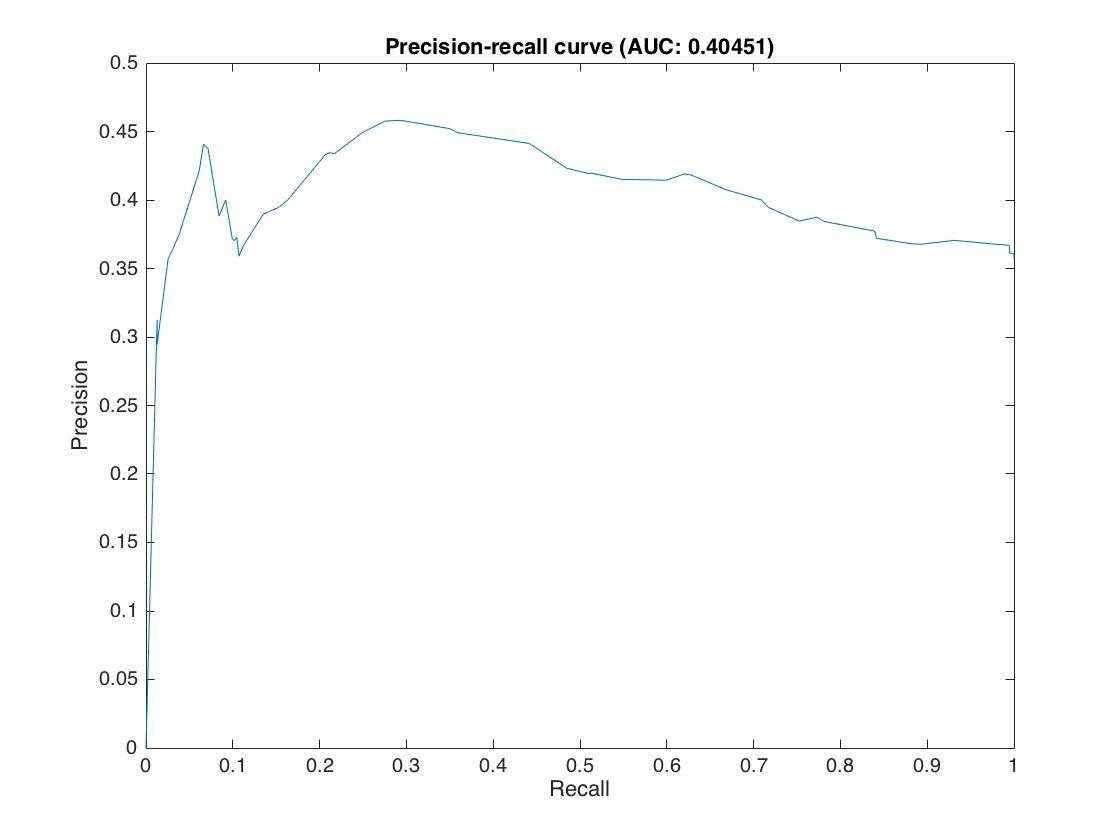
\includegraphics[width=0.85\textwidth]{train_dsi_test_dso_prec_rec}
    \caption{The Precision-Recall curve for DSO-1 cross-validation}
    \label{fig:train_dsi_test_dso}
\end{figure}

\subsubsection{Test case 4: cross dataset performance on DSI-1}


\begin{figure}[h!]
  \centering
    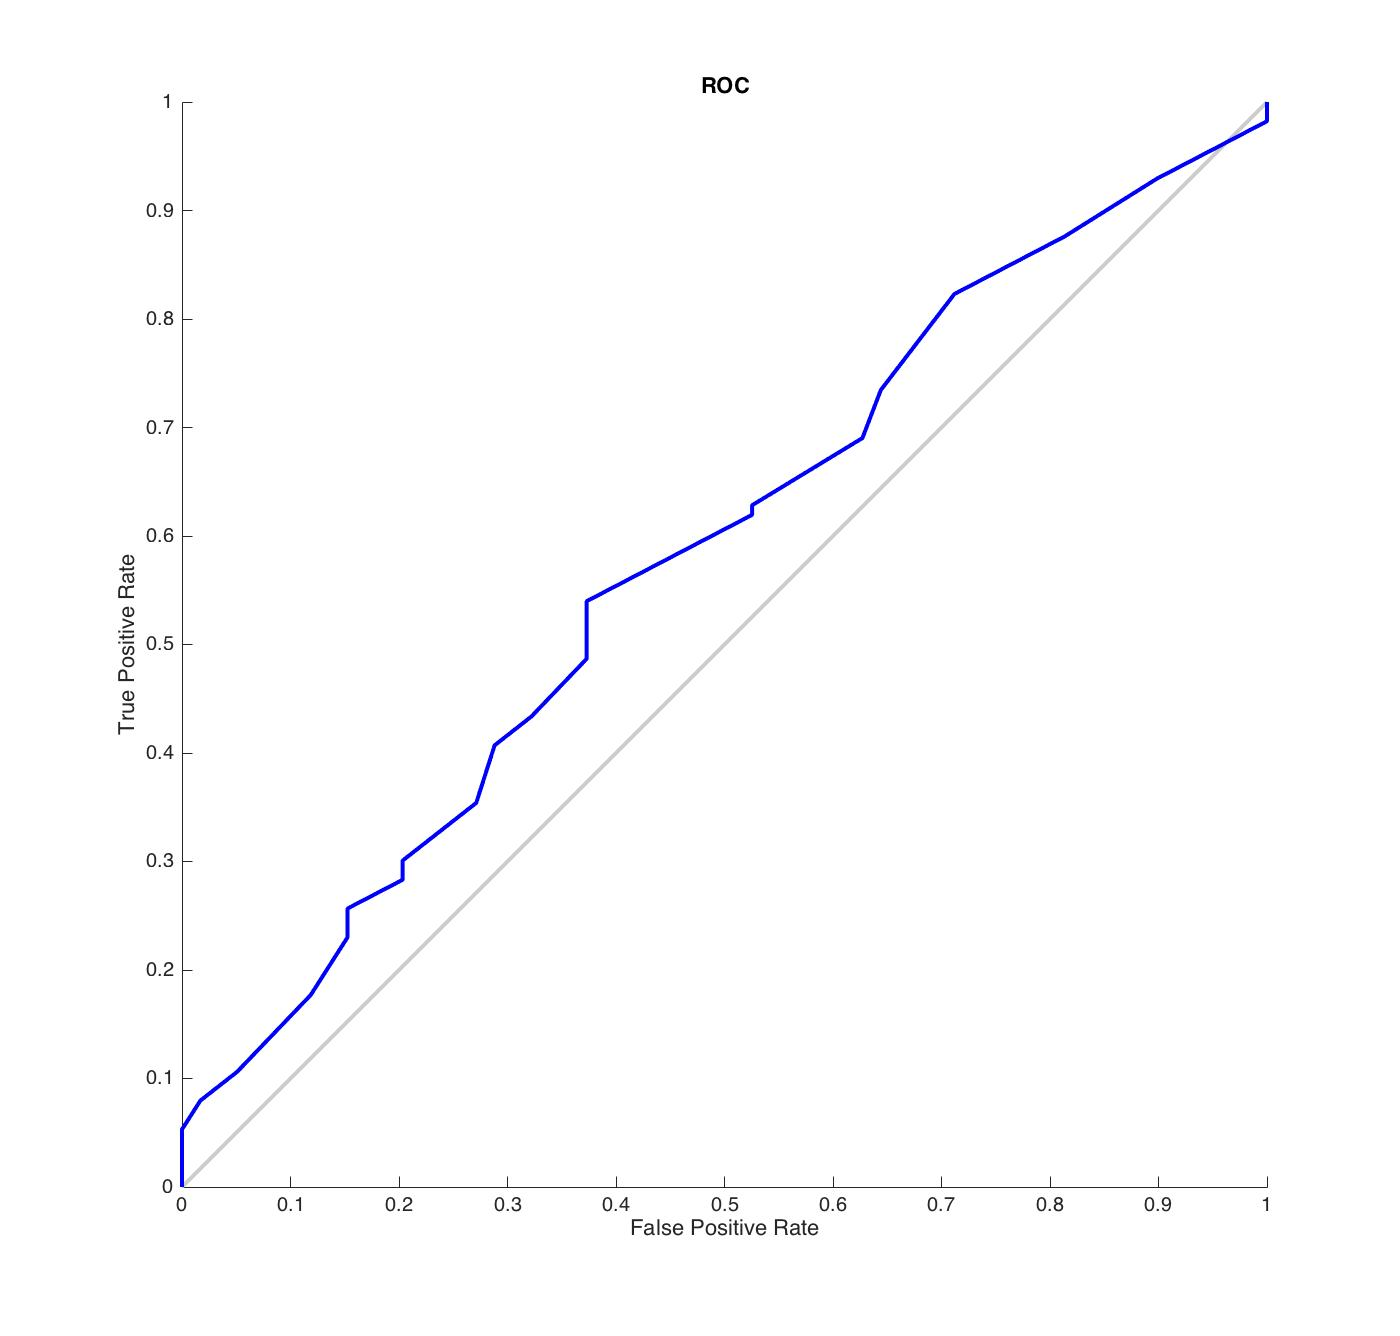
\includegraphics[width=0.85\textwidth]{train_dso_test_dsi}
    \caption{The ROC curve  for DSI-1 cross-validation}
    \label{fig:train_dso_test_dsi}
\end{figure}

\begin{figure}[h!]
  \centering
    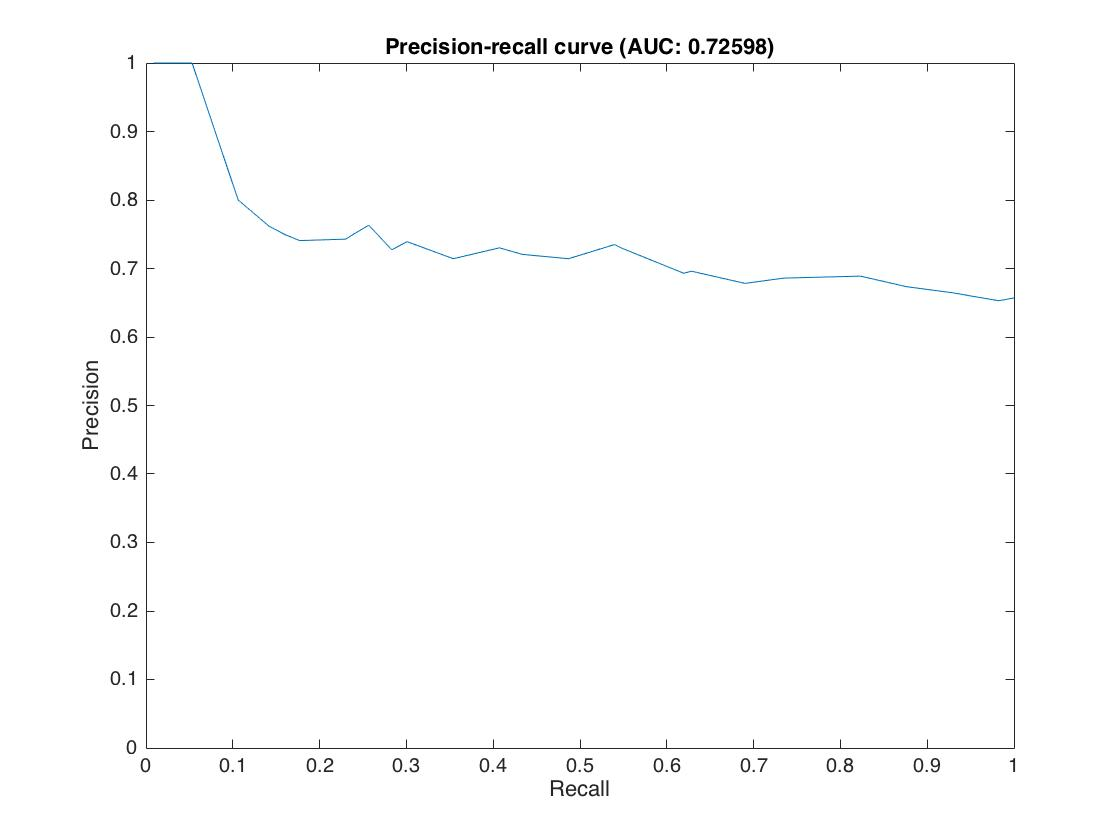
\includegraphics[width=0.85\textwidth]{train_dso_test_dsi_prec_rec}
    \caption{The Precision-Recall curve for DSI-1 cross-validation}
    \label{fig:train_dso_test_dsi_prec_rec}
\end{figure}

\section{Regions forgery detection module performance}


In the classification stage, we used a 10-fold cross validation protocol, an SVM classifier with an RBF
kernel, and classical grid search for adjusting parameters in training samples \cite{bishop2007pattern}.



